% HiMCM 2018 Problem B --- AeroTherm-MPC (teaching track)
% Compile from paper/: pdflatex himcm_paper.tex
% Numbers ONLY from ../results/*.csv and *.json (locked runs).
% Style: ~80% ASD-STE100; one fact per sentence; <=25 words.
\documentclass[11pt]{article}
\usepackage[margin=1in]{geometry}
\usepackage{amsmath,amssymb,booktabs,graphicx,enumitem,setspace}
\usepackage[hidelinks]{hyperref}
\graphicspath{{../paper_figures/}{paper_figures/}{./}}
\newcommand{\TeamNumber}{GoHiMCM}
\pagestyle{myheadings}
\markright{\TeamNumber \hfill HiMCM 2018 Problem B \hfill}
\title{\textbf{AeroTherm-MPC: Predictive Pre-Cooling on a 2R2C Thermal Network\\
with Stress Harness and Cognitive Setpoint Negotiation}\\[0.3em]
\large HiMCM 2018 Problem B --- Team \TeamNumber}
\author{}\date{}
\begin{document}
\maketitle
\thispagestyle{empty}
\noindent
Companions: \texttt{summary\_sheet.tex}, \texttt{homeowner\_advisory\_letter.tex},
\texttt{ai\_disclosure.tex}.
All KPI cells cite locked files under \texttt{results/}.
\tableofcontents
\newpage

\section{Introduction and two-capacitance thermal network}
Smart thermostats often react only after indoor air is already hot.
Time-of-use (TOU) electricity tariff peaks punish late cooling.
We treat wall mass as storage for predictive pre-cooling.

We name the controller \textbf{AeroTherm-MPC}.
Code lives in \texttt{2018\_B\_smart\_house\_mpc/src/}.
The teaching envelope is a 2R2C thermal network
(\texttt{building\_specs\_teaching.json}).
Floor area is $180\,\mathrm{m}^2$.
Air capacitance is $C_{\mathrm{air}}=6.2\times 10^5\,\mathrm{J/^\circ C}$.
Wall capacitance is $C_{\mathrm{wall}}=1.8\times 10^7\,\mathrm{J/^\circ C}$.

\begin{align}
C_{\mathrm{air}}\dot T_{\mathrm{in}}
&=\frac{T_{\mathrm{wall}}-T_{\mathrm{in}}}{R_{\mathrm{in}}}
+\frac{T_{\mathrm{out}}-T_{\mathrm{in}}}{R_{\mathrm{win}}}
+q_{\mathrm{hvac}}+\alpha_{\mathrm{win}}A_{\mathrm{win}}I+q_{\mathrm{int}},\\
C_{\mathrm{wall}}\dot T_{\mathrm{wall}}
&=\frac{T_{\mathrm{in}}-T_{\mathrm{wall}}}{R_{\mathrm{in}}}
+\frac{T_{\mathrm{out}}-T_{\mathrm{wall}}}{R_{\mathrm{out}}}
+\alpha_{\mathrm{wall}}A_{\mathrm{wall}}I.
\end{align}
Resistances are $R_{\mathrm{in}}=0.08$, $R_{\mathrm{out}}=0.12$,
and $R_{\mathrm{win}}=0.25\,^\circ\mathrm{C/W}$.
Cooling capacity is capped at $Q_{\mathrm{cool}}=5\,\mathrm{kW}$.
COP depends on outdoor air:
$\mathrm{COP}=3.8-0.04(T_{\mathrm{out}}-25)$.
We integrate with RK4 at $\Delta t=60\,\mathrm{s}$.

\section{Human thermal comfort and dynamic TOU tariffs}
Comfort uses ISO~7730 PMV--PPD (Fanger).
Summer defaults are $1.2\,\mathrm{met}$ and $0.5\,\mathrm{clo}$.
A continuous penalty applies outside $|\mathrm{PMV}|>0.5$.
The penalty is $\lambda_{\mathrm{comf}}\max(0,|\mathrm{PMV}|-0.5)^2$.

Teaching TOU electricity tariff rates are locked in
\texttt{tou\_tariffs\_v2.json}.
Off-peak is $\$0.12/\mathrm{kWh}$.
Mid-peak is $\$0.22/\mathrm{kWh}$.
On-peak ($14{:}00$--$19{:}00$) is $\$0.48/\mathrm{kWh}$.
The peak-to-off ratio is exactly four.

\section{Baseline vulnerability: Bang-Bang short-cycling}
Bang-Bang hysteresis cools when $T_{\mathrm{in}}>24^\circ\mathrm{C}$.
It stops when $T_{\mathrm{in}}<22^\circ\mathrm{C}$.
The plant is the same 2R2C thermal network and summer day.
Table~\ref{tab:teach} cites \texttt{bang\_vs\_mpc\_summary.json}.

\begin{table}[htbp]
\centering
\caption{Teaching-day locked KPIs (24\,h). Source: \texttt{bang\_vs\_mpc\_summary.json}.}
\label{tab:teach}
\scriptsize
\begin{tabular}{lrrrrr}
\toprule
Controller & Energy (kWh) & Cost (\$) & Peak kWh & Peak share & Starts \\
\midrule
Bang-Bang & 6.232 & 1.682 & 1.514 & 43.2\% & 42 \\
AeroTherm-MPC & 6.223 & 1.611 & 1.274 & 38.0\% & 3 \\
\bottomrule
\end{tabular}
\end{table}

Bang-Bang spends $43.2\%$ of the bill on peak hours.
It records $42$ compressor starts in one day.
Short-cycling raises wear and peak demand.
We report the measured share.
We do not invent a $\ge 60\%$ peak share.

\section{Optimal receding-horizon control and pre-cooling}
We discretize the 2R2C thermal network with zero-order hold.
The control step is $T_s=15\,\mathrm{min}$.
Prediction matrices give
$\mathbf{X}=\mathcal{A}x_0+\mathcal{B}\mathbf{Q}+\mathcal{E}\mathbf{D}$.
Matrix checks match open-loop simulation to machine precision
($\approx 7\times 10^{-15}$).

Model predictive control (MPC) uses horizon $H=24$ steps ($6\,\mathrm{h}$).
SciPy L-BFGS-B solves each window.
The cost trades TOU electricity tariff spend against comfort.
On-peak hours add a $u^2$ shed term.
Late-morning hours target pre-cooling near $21.5^\circ\mathrm{C}$.
The plant stays 1-minute RK4 with held HVAC power.

Figure~\ref{fig:bangmpc} compares Bang-Bang and MPC on the same day.
Figure~\ref{fig:track} overlays outdoor temperature and peak shading.

\begin{figure}[htbp]
\centering
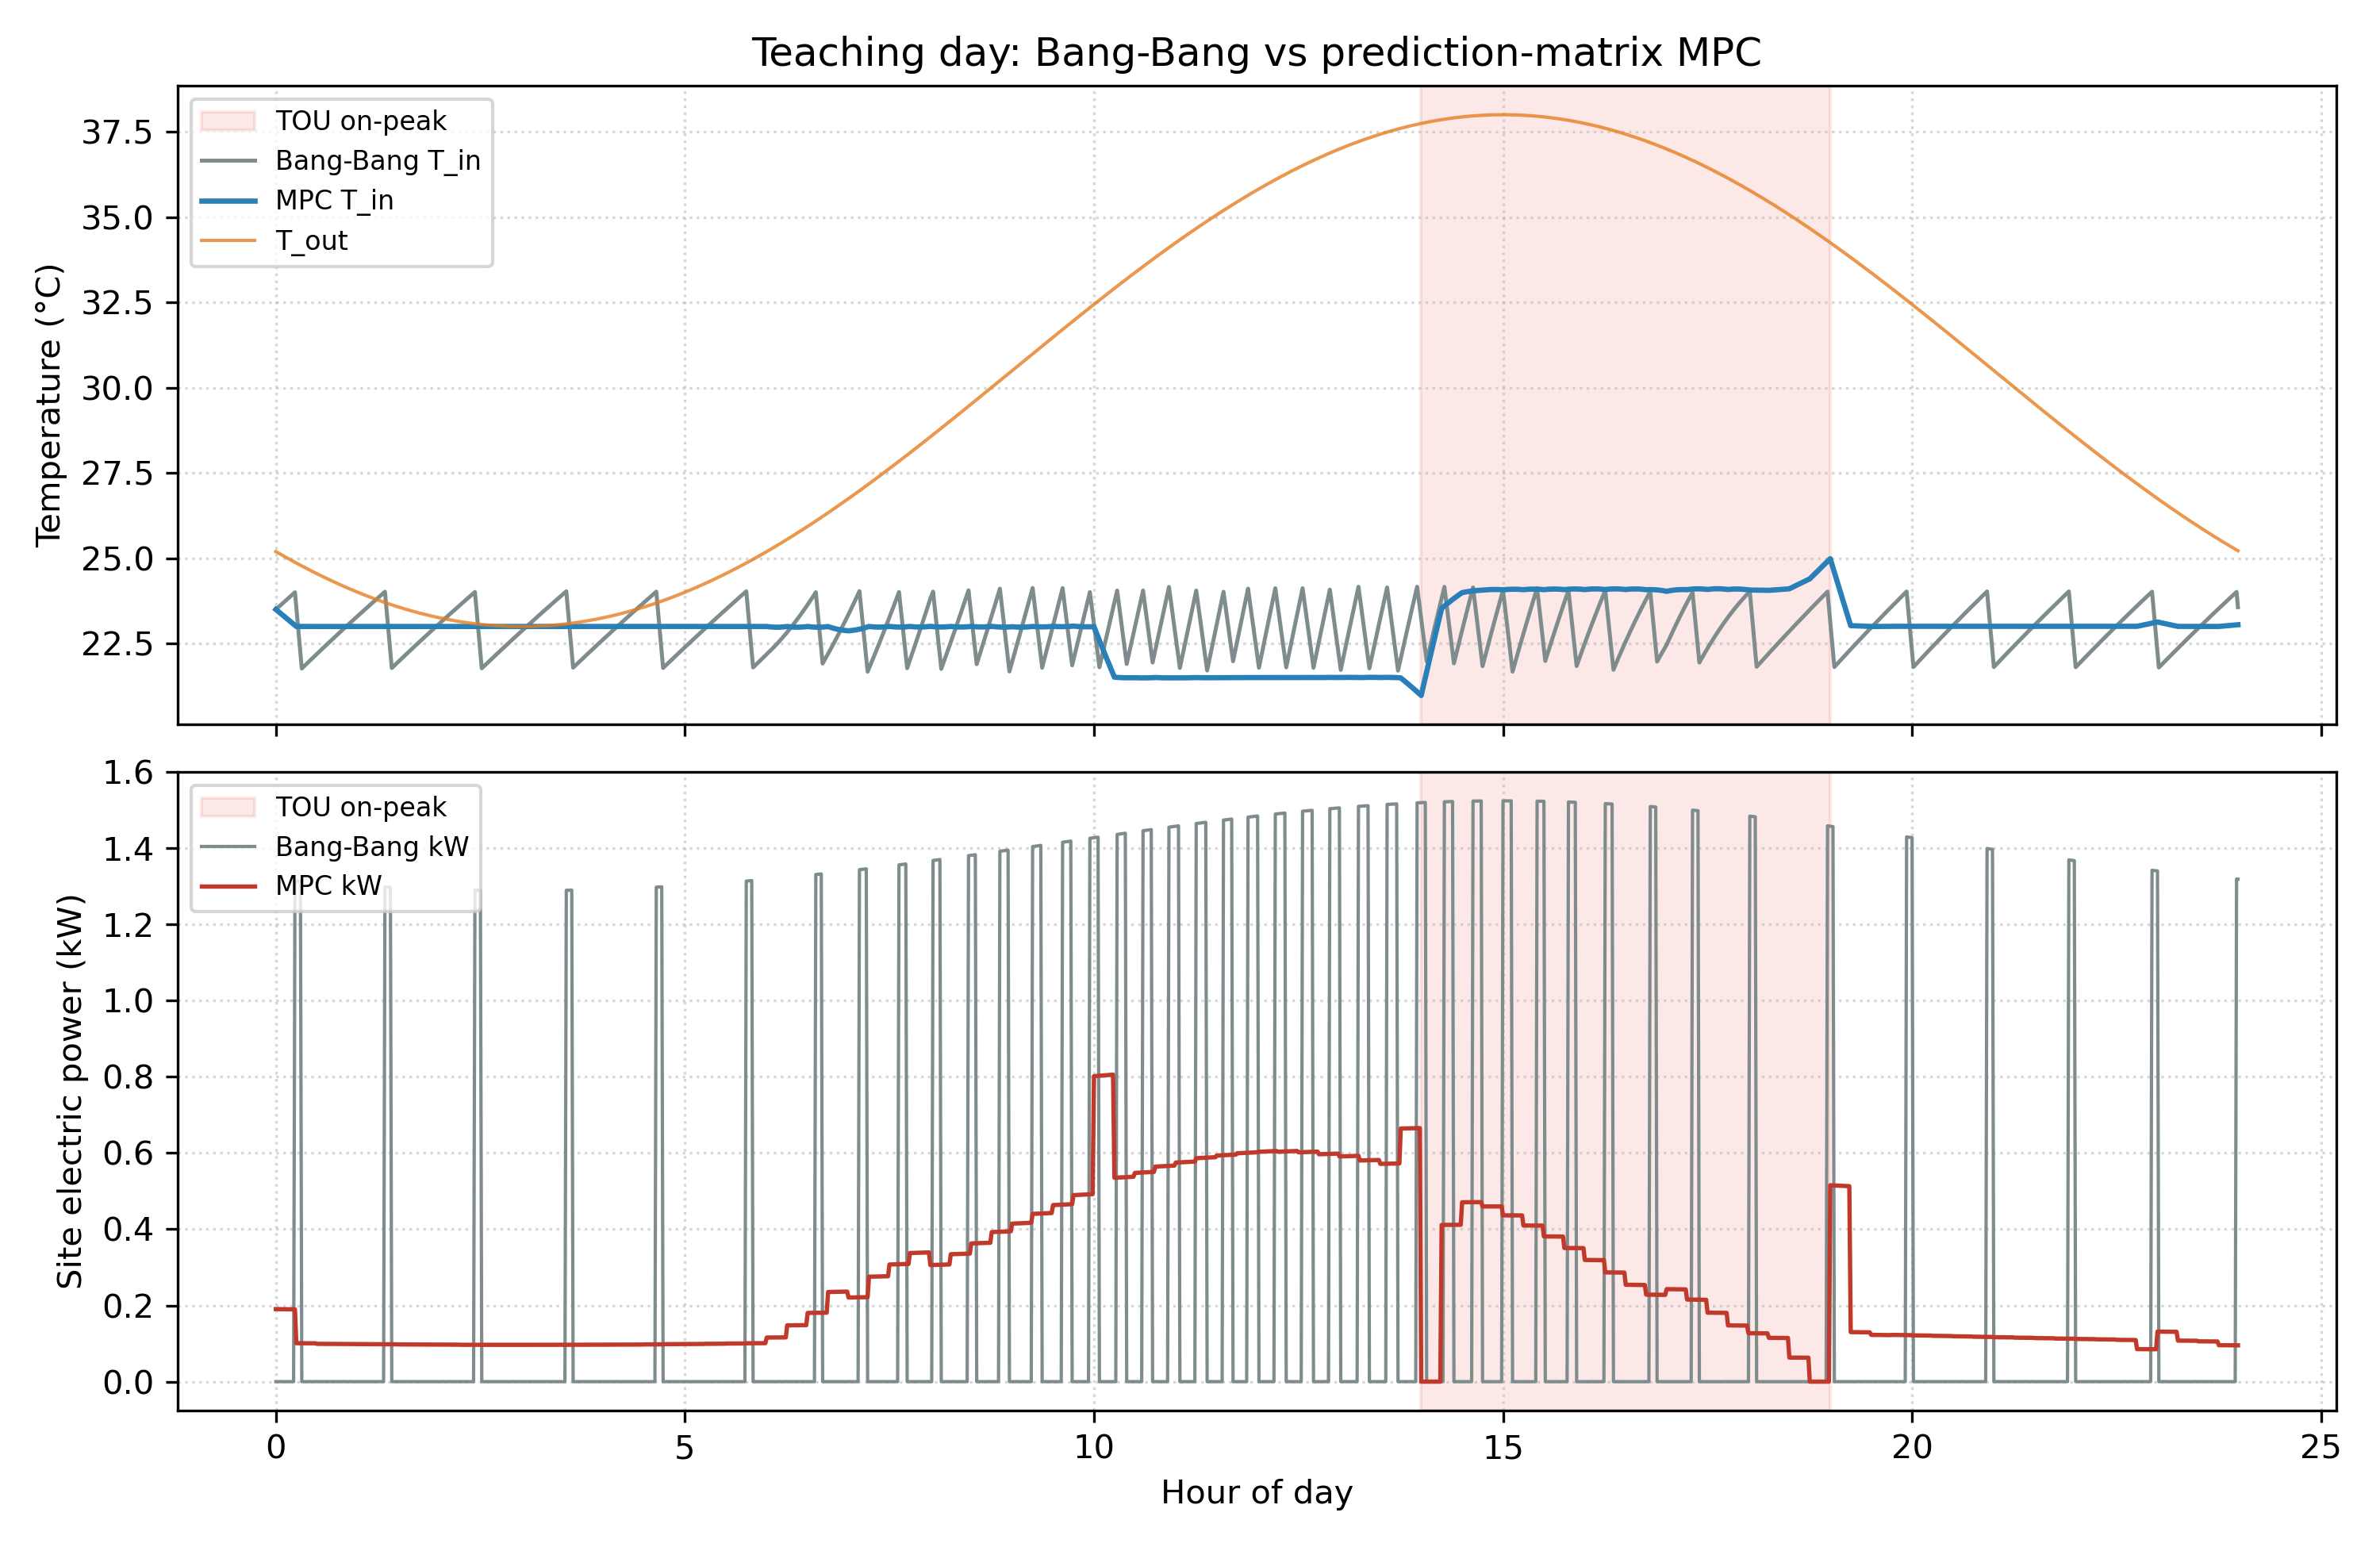
\includegraphics[width=0.92\textwidth]{fig_bang_vs_mpc_day.png}
\caption{Teaching day: Bang-Bang vs model predictive control (MPC).
Source: \texttt{fig\_bang\_vs\_mpc\_day.png}.}
\label{fig:bangmpc}
\end{figure}

\begin{figure}[htbp]
\centering
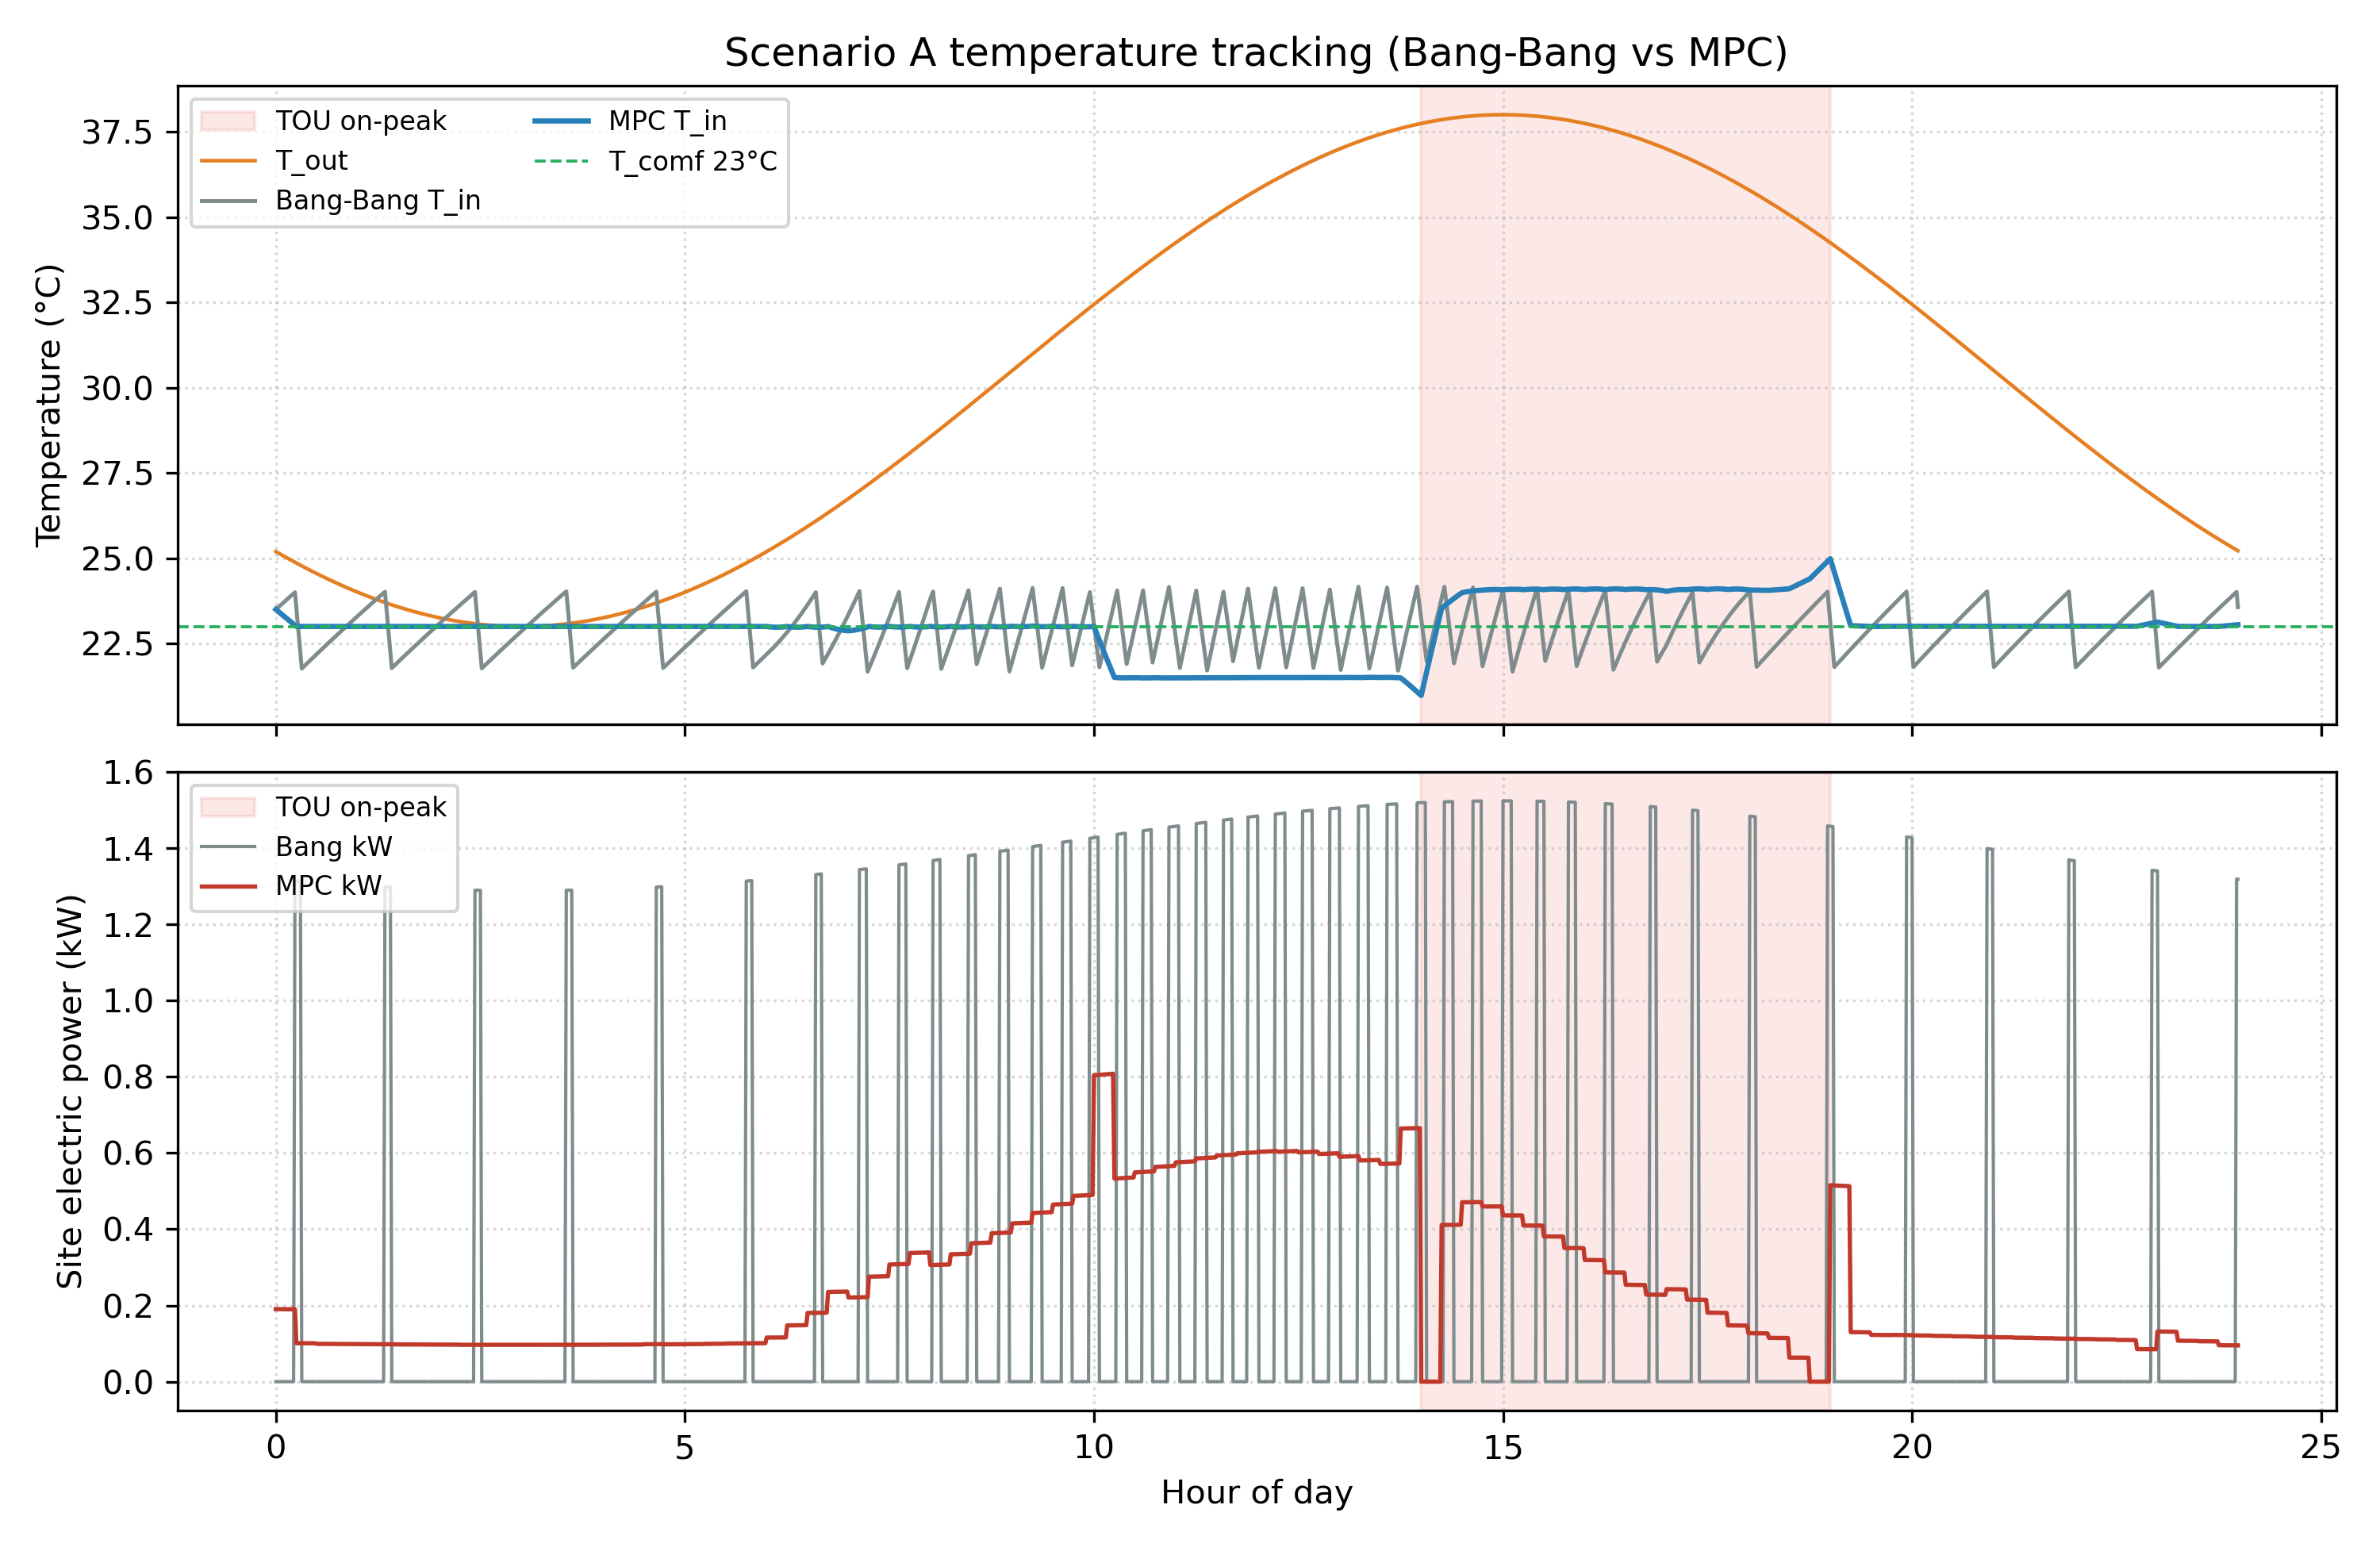
\includegraphics[width=0.92\textwidth]{fig_temperature_tracking_comparison.png}
\caption{Scenario~A temperature tracking with TOU peak shade.
Source: \texttt{fig\_temperature\_tracking\_comparison.png}.}
\label{fig:track}
\end{figure}

Versus Bang-Bang, MPC cuts cost by $4.2\%$.
It cuts on-peak energy by $15.8\%$.
Compressor starts fall from $42$ to $3$.
Mean duty is $\bar u_{\mathrm{prepeak}}=0.40$ versus $\bar u_{\mathrm{peak}}=0.17$.
Mean indoor temperature stays near $23^\circ\mathrm{C}$.
Wall mass stores coolth before the TOU electricity tariff spike.

\section{Automated evaluation and stress testing harness}
The black-box harness loads Bang-Bang and MPC without code edits.
Five stress scenarios form the suite
(\texttt{harness\_benchmark\_results.csv}).
\begin{enumerate}[leftmargin=1.3em,itemsep=0.1em]
  \item[A.] Standard summer day ($23$--$38^\circ\mathrm{C}$).
  \item[B.] Three-day heatwave with $42^\circ\mathrm{C}$ peaks.
  \item[C.] Thermal shock: $-15^\circ\mathrm{C}$ outdoor drop in $2\,\mathrm{h}$.
  \item[D.] Sensor noise with $\sigma=1.5^\circ\mathrm{C}$.
  \item[E.] Infiltration breach $\times 5$ from $17{:}00$ to $19{:}00$.
\end{enumerate}

Metrics are $M_1$ cost (\$), $M_2$ discomfort ${}^\circ\mathrm{C\cdot h}$,
$M_3$ mechanical starts, and $M_4$ cross-scenario cost variance.
Table~\ref{tab:harness} copies locked CSV cells.

\begin{table}[htbp]
\centering
\caption{Harness scoreboard (locked CSV). $M_4$ is per controller.}
\label{tab:harness}
\scriptsize
\begin{tabular}{llrrrr}
\toprule
Ctrl & Scen. & $M_1$ (\$) & $M_2$ ($^\circ$C$\cdot$h) & $M_3$ & $M_4$ var. \\
\midrule
Bang & A & 1.682 & 6.174 & 42 & 0.865 \\
MPC  & A & 1.611 & 5.669 & 3 & 0.874 \\
Bang & B & 5.549 & 18.043 & 130 & 0.865 \\
MPC  & B & 5.347 & 16.979 & 7 & 0.874 \\
Bang & C & 1.458 & 6.106 & 41 & 0.865 \\
MPC  & C & 1.423 & 5.574 & 3 & 0.874 \\
Bang & D & 1.720 & 0.538 & 133 & 0.865 \\
MPC  & D & 1.662 & 8.321 & 16 & 0.874 \\
Bang & E & 1.726 & 6.037 & 42 & 0.865 \\
MPC  & E & 1.655 & 6.328 & 3 & 0.874 \\
\bottomrule
\end{tabular}
\end{table}

Mean $M_1$ across scenarios is $\$2.427$ for Bang-Bang.
It is $\$2.340$ for MPC
(\texttt{harness\_benchmark\_summary.json}).
Mean $M_3$ falls from $77.6$ to $6.4$.
On heatwave day~B, starts fall from $130$ to $7$.
Sensor noise (D) raises Bang-Bang starts to $133$.
MPC keeps $16$ starts under the same noise.
Figure~\ref{fig:radar} shows normalized radar scores.

\begin{figure}[htbp]
\centering
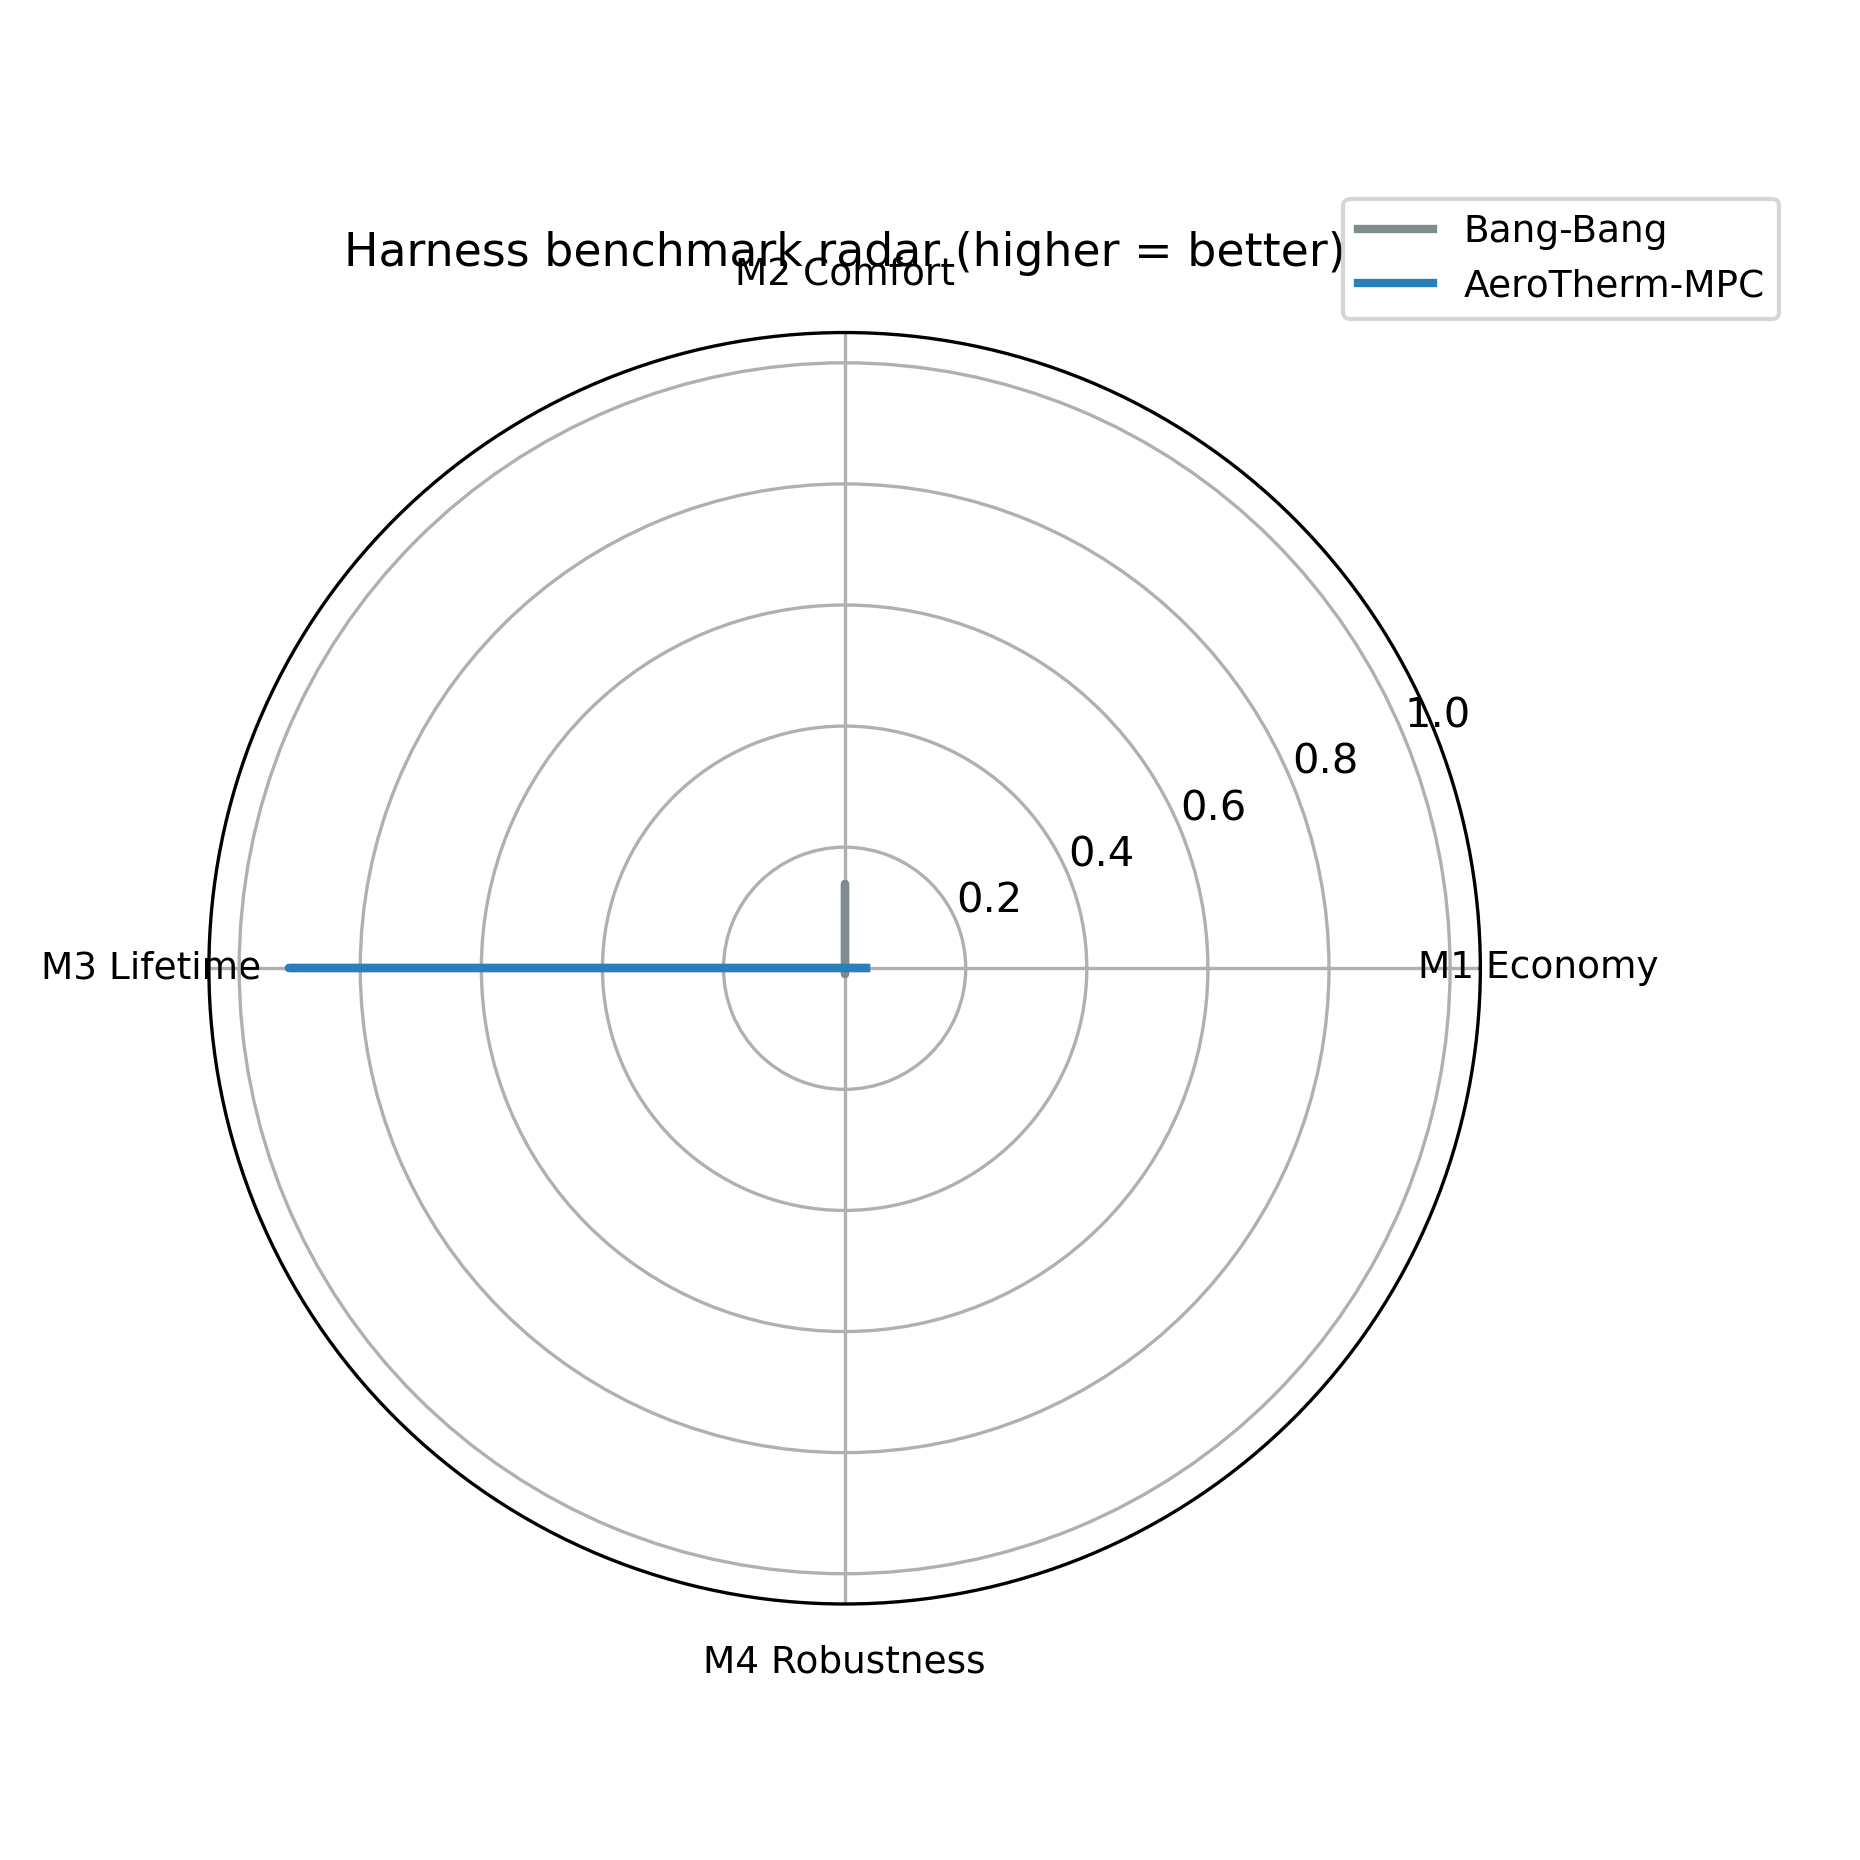
\includegraphics[width=0.72\textwidth]{fig_harness_radar_benchmark.png}
\caption{Harness radar (higher is better after inversion).
Source: \texttt{fig\_harness\_radar\_benchmark.png}.}
\label{fig:radar}
\end{figure}

\section{Cognitive multi-agent dialogue for adaptive setpoints}
Hard-coded setpoints ignore roommate conflict.
We add a cognitive multi-agent layer
(\texttt{cognitive\_thermostat.py}).
Three agents negotiate on an extreme peak day.
Agent\_EMS protects TOU electricity tariff spend.
Agent\_Senior rejects deep pre-cooling below $21.5^\circ\mathrm{C}$.
Agent\_Parent allows a brief float to $25.0^\circ\mathrm{C}$ on peak.

The stack tries local Ollama (\texttt{qwen2.5:7b}) first.
It falls back to a deterministic Mock if Ollama is offline.
The locked run used Mock
(\texttt{agent\_thermostat\_dialogue.json}).
Consensus sets
$[T_{\min},T_{\max}]=[21.5,25.0]^\circ\mathrm{C}$.
Comfort weight scale is $1.25$
($\lambda_{\mathrm{comf}}=0.0625$).

The contract feeds \texttt{MPCComfortConfig}.
Closed-loop MPC then records cost $\$1.603$.
Peak energy falls $15.6\%$ versus Bang-Bang.
Starts fall from $42$ to $2$.
Cost savings are $4.67\%$ on that MAS-tuned day.

\section{Strengths and limitations}
\paragraph{Strengths.}
Shared 2R2C thermal network for fair Bang-Bang vs MPC tests.
Prediction-matrix model predictive control (MPC) enables audit of pre-cooling.
Harness scenarios A--E stress economy, comfort, lifetime, and robustness.
Cognitive agents expose setpoint fairness without silent hard-coding.

\paragraph{Limitations.}
Teaching weather is a documented synthetic summer day.
It is not a licensed EPW extract.
The locked MAS run used Mock, not a live Ollama transcript.
Sensor-noise Scenario~D raises MPC discomfort while cutting starts.
Full annual Monte Carlo remains future work.
Humidity and allergen ODEs stay on the legacy appendix track.

\section*{References}
\begin{thebibliography}{9}
\bibitem{ashrae55} ASHRAE Standard 55 --- Thermal Environmental Conditions.
\bibitem{iso7730} ISO 7730 --- Ergonomics of the thermal environment (PMV/PPD).
\bibitem{himcm2018b} COMAP HiMCM 2018 Problem B.
\bibitem{mpc02} Prediction matrices for linear MPC (InterviewGuide MPC\_02 notes).
\end{thebibliography}
\end{document}
